%
% File acl2014.tex
%
% Contact: koller@ling.uni-potsdam.de, yusuke@nii.ac.jp
%%
%% Based on the style files for ACL-2013, which were, in turn,
%% Based on the style files for ACL-2012, which were, in turn,
%% based on the style files for ACL-2011, which were, in turn, 
%% based on the style files for ACL-2010, which were, in turn, 
%% based on the style files for ACL-IJCNLP-2009, which were, in turn,
%% based on the style files for EACL-2009 and IJCNLP-2008...

%% Based on the style files for EACL 2006 by 
%%e.agirre@ehu.es or Sergi.Balari@uab.es
%% and that of ACL 08 by Joakim Nivre and Noah Smith

\documentclass[11pt]{article}

\usepackage{acl2014}

\usepackage{times}

\usepackage{url}

\usepackage{latexsym}

\usepackage{graphicx}

\usepackage{amssymb}

\newcommand{\me}{\mathrm{e}}

%\setlength\titlebox{5cm}

% You can expand the titlebox if you need extra space
% to show all the authors. Please do not make the titlebox
% smaller than 5cm (the original size); we will check this
% in the camera-ready version and ask you to change it back.


\title{Learning Abstract Concepts from Multi-Modal Data: \\ Since You Probably Can't See What I Mean}

\author{First Author \\
  Affiliation / Address line 1 \\
  Affiliation / Address line 2 \\
  Affiliation / Address line 3 \\
  {\tt email@domain} \\\And
  Second Author \\
  Affiliation / Address line 1 \\
  Affiliation / Address line 2 \\
  Affiliation / Address line 3 \\
  {\tt email@domain} \\}


\date{}


\begin{document}

\maketitle

\begin{abstract}



Models that acquire semantic representations from both linguistic and perceptual input outperform linguistic-only models on various NLP tasks. However, this superiority has only been established when learning concrete concepts, which are usually domain specific and also comparatively rare in everyday language. We extend the scope to more widely applicable abstract representations, and present  a multi-modal probabilistic language architecture for learning semantic representations for both concrete and abstract concepts. Our model outperforms alternative approaches in combining input from two modalities and also in propagating perceptual information on concrete to more abstract concepts. We discuss the implications of our results both for optimizing the performance of multi-modal models and for theories of abstract conceptual representation. 




\end{abstract}



\section{Introduction}

Multi-modal models that learn semantic representations from both language and information about the perceptible properties of concepts were originally motivated by parallels with human word learning \cite{andrews2009integrating} and evidence that many concepts are grounded in perception \cite{barsalou2005situating}. The perceptual information in such models is generally mined directly from images \cite{feng2010visual,bruni2012distributional} or from data collected in psychological studies \cite{silberer2012grounded,rollermultimodal}. 

By exploiting the additional information encoded in perceptual input, multi-modal models can outperform language-only models on a range of semantic NLP tasks, including modelling similarity \cite{bruni2014multimodal} and free association \cite{silberer2012grounded}, predicting compositionality \cite{rollermultimodal} and concept categorization \cite{silberer2014learning}. However, to date, this superiority has only been established when evaluating on concrete words such as \emph{cat} or \emph{dog}, rather than abstract concepts, such as \emph{curiosity} or \emph{loyalty}. Indeed, differences between abstract and concrete processing and representation \cite{paivio1991dual,hill2013quantitative} suggest that conclusions about concrete concept learning may not necessarily hold in the general case. In this paper, we therefore focus on multi-modal models for learning both abstract and concrete concepts.

Although concrete concepts might seem more basic or fundamental, the vast majority of open-class, meaning-bearing words in everyday language are in fact abstract. 72\% of the noun or verb tokens in the British National Corpus \cite{leech1994claws4} are rated by human judges\footnote{Contributors to the USF dataset \cite{nelson2004university}} as more abstract than the noun \emph{war}, for instance, a concept many would already consider to be quite abstract. Moreover, abstract concepts by definition encode higher-level (more general) principles than concrete concepts, which typically reside naturally in a single semantic category or domain \cite{crutch2005abstract}. It is therefore likely that abstract representations may prove highly applicable for multi-task, multi-domain or transfer learning models, which aim to acquire `general-purpose' conceptual knowledge without reference to a specific objective or task \cite{collobert2008unified,mesnil2012unsupervised}. 

Motivated by these observations, we introduce an architecture for learning both abstract and concrete representations that generalizes the skipgram model of \newcite{mikolov2013efficient} from corpus-based  to multi-modal learning. The extended model is designed to reflect aspects of human word learning, in that it introduces more perceptual information about commonly-occurring concrete concepts and less information about rarer concepts. 

We train our model on running-text language and two sources of perceptual descriptors for concrete nouns: the ESPGame dataset of annotated images \cite{von2004labeling} and the CSLB set of concept property norms \cite{devereux2013centre}. We find that our model \emph{combines} information from the different modalities more effectively than previous methods, resulting in an improved ability to model the USF free association gold standard \cite{nelson2004university} for concrete nouns. In addition, the architecture  \emph{propagates} the extra-linguistic input for concrete nouns to improve representations of abstract concepts more effectively than alternative methods. While this propagation can effectively extend the advantage of the multi-modal approach to many more concepts than simple concrete nouns, we observe that the benefit of adding perceptual input appears to decrease as target concepts become more abstract. Indeed, for the most abstract concepts of all, language-only models still provide the most effective learning mechanism.  

Finally, we investigate the optimum quantity and type of perceptual input for such models. Between the most concrete concepts, which can be effectively represented directly in the perceptual modality, and the most abstract concepts, which cannot, we identify a set of concepts that cannot be represented effectively directly in the perceptual modality, but still benefit from perceptual input propagated in the model via concrete concepts. 

The motivation in designing our model and experiments is both practical and theoretical. Taken together, the empirical observations we present are potentially important for optimizing the learning of representations of concrete and abstract concepts in multi-modal models. In addition, they offer a degree of insight into the poorly understood issue of how abstract concepts may be encoded in human memory.    

\section{Model Design}

Before describing how our multi-modal architecture encodes and integrates perceptual information, we first describe the underlying corpus-based representation learning model. 

\paragraph{Language-only Model} Our multi-modal architecture builds on the continuous log-linear skip-gram language model proposed by \newcite{mikolov2013efficient}. This model learns lexical representations in a similar way to neural-probabilistic language models (NPLM) but without a non-linear hidden layer, a simplification that facilitates the efficient learning of large vocabularies of dense representations, generally referred to as \emph{embeddings} \cite{turian2010word}. Embeddings learned by the model achieve state-of-the-art performance on several evaluations including sentence completion and analogy modelling \cite{mikolov2013efficient}.   

\begin{figure*}[ht]  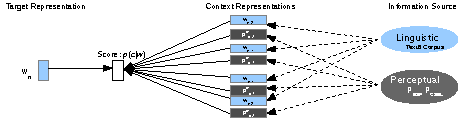
\includegraphics[width = \textwidth]{Figure_1}  \caption{Our multi-modal model architecture. Light boxes are elements of the original \newcite{mikolov2013efficient} model. For target words \(w_n\) in the domain of \(\mathbf{P}\), the model updates based on corpus context words \( w_{n+i} \) then on words \(p^w_{n+i}\) in perceptual psuedo-sentences. Otherwise, updates are based solely on the \( w_{n+i}. \)}\end{figure*}

For each word type \(w\) in the vocabulary \(V\), the model learns both a `target-embedding' \( r_{w} \in \mathbb{R}^d\) and a `context-embedding' \(\hat{r}_{w} \in \mathbb{R}^d\) such that, given a target word, its ability to predict nearby context words is maximized. The probability of seeing context word \(c\) given target \(w\) is defined as:  

\[p(c|w)  = \frac{\me^{\hat{r}_{c} \cdot r_{w}}}{\sum_{v \in V} \me^{\hat{r}_v\cdot r_{w}}}    \] 

The model learns from a set of target-word, context-word pairs, extracted from a corpus of sentences as follows. In a given sentence \(S\) (of length \(N\)), for each position \( n \leq N\), each word \(w_n\) is treated in turn as a target word. An integer \( {t(n)} \) is then sampled from a uniform distribution on \( \{1, \dots k \} \), where \(k > 0\) is a predefined maximum context-window parameter. The pair tokens \( \{(w_n, w_{n+j}): -{t(n)}\leq j \leq {t(n)}, w_i \in S \}\) are then appended to the training data. Thus, target/context training pairs are such that (i) only words within a \(k\)-window of the target are selected as context words for that target, and (ii) words closer to the target are more likely to be selected than those further away.

The training objective is then to maximize the log probability \( T\) across of all such examples from \(S\), and then across all sentences in the corpus:
 
\[ T = \frac{1}{N} \sum_{n=1}^{N} \sum_{-{t(n)}\leq j \leq {t(n)}, j\neq 0} log(  p(w_{n+j}|w_{n}) ) \]The model free parameters (target-embeddings and context-embeddings of dimension \(d\) for each word in the corpus with frequency above a certain threshold \(f\)) are updated according to stochastic gradient descent and backpropation, with learning rate controlled by Adagrad \cite{duchi2011adaptive}. For efficiency, the output layer is encoded as a hierarchical softmax function based on a binary Huffman tree \cite{morin2005hierarchical}. 

As with other distributional architectures, the model captures conceptual semantics by exploting the fact that words appearing in similar linguistic contexts are likely to have similar meanings. Informally, the model adjusts its embeddings to increase the `probability' of seeing the language in the training corpus. Since this probability increases with the \(p(c|w)\), and the \(p(c|w)\) increase with the dot product \( \hat{r}_v\cdot r_{c} \), the updates have the effect of moving each target-embedding incrementally `closer' to the context-embeddings of its collocates. In the target-embedding space, this results in embeddings of concept words that regularly occur in similar contexts moving closer together.   


\paragraph{Multi-modal Extension} We extend the \newcite{mikolov2013efficient} architecture via a simple means of introducing perceptual information that aligns with human language learning. Based on the assumption that frequency in domain-general linguistic corpora correlates with the likelihood of `experiencing' a concept in the world \cite{bybee2001frequency,chater2006probabilistic}, perceptual information is introduced to the model whenever designated concrete concepts are encountered in the running-text linguistic input. This has the effect of introducing more perceptual input for commonly experienced concrete concepts and less input for rarer concrete concepts. 

To implement this process,  perceptual information is extracted from external sources and encoded in an associative array \(\bf{P}\), which maps (typically concrete) words \(w\) to bags of perceptual features \({\bf b}(w)\). The construction of this array depends on the perceptual information source; the process for our chosen sources is detailed in Section 2.1.  

Training our model begins as before on running-text. When a sentence \(S_m\) containing a word \(w\) in the domain of \(\mathbf{P}\) is encountered, the model completes training on \(S_m\) and begins learning from a perceptual pseudo-sentence \(\hat{S}(w)\).  \(\hat{S_m}(w)\) is constructed  by randomly sampling features from \({\bf b}(w)\) to occupy positions before and instances of \(w\), so that  \(\hat{S_m}(w)\) is the same length as \(S_m\) (see Figure 2). Once training on \(\hat{S_m}(w)\) is completed, the model reverts to the next `real' (linguistic) sentence \(S_{m+1}\), and the process continues. Thus, when a concrete concept is encountered in the corpus, its embedding is first updated based on language (moved incrementally closer to concepts appearing in similar linguistic contexts), and then on perception (moved incrementally closer to concepts with the same or similar perceptual features).  

For greater flexibility, we introduce a parameter \(\alpha\) reflecting the raw quantity of perceptual information relative to linguistic input. When \(\alpha=2\), two pseudo-sentences are generated and inserted for every corpus occurrence of a token from the domain of \(\mathbf{P}\). For non-integral \(\alpha \), the number of sentences inserted is \( \lfloor \alpha \rfloor \), and a further sentence is added with probability \(\alpha - \lfloor \alpha \rfloor \).

In all experiments reported in the following sections we set the window size parameter \(k = 5\) and the minimum frequency parameter \(f = 3\), which guarantees that the model learns embeddings for all concepts in our evaluation sets. While the model learns both target and context-embeddings for each word in the vocabulary, we conduct our experiments with the target embeddings only. We set the dimension parameter \(d = 300 \) as this produces high quality embeddings in the language-only case \cite{mikolov2013efficient}. 

\begin{figure} \(\hat{S}(crocodile) =\)\small{ {\bf Crocodile} legs {\bf crocodile} teeth {\bf crocodile} teeth {\bf crocodile} scales {\bf crocodile} green {\bf crocodile}. \\ \\ \(\hat{S}(screwdriver)=\) { \bf Screwdriver} handle {\bf screwdriver} flat  {\bf screwdriver} long {\bf screwdriver}  handle {\bf screwdriver}  head. } \caption{Example pseudo-sentences generated by our model.}\end{figure}

\subsection{Information Sources}

We construct the associative array of perceptual information \(\mathbf{P}\) from two sources typical of those typically used for multi-modal semantic models.

\paragraph{ESPGame Dataset} The ESP-Game dataset (ESP) \cite{von2004labeling} consists of 100,000 images, each annotated with a list of lexical concepts that appear in that image.  

For any concept \(w\) identified in an ESP image, we construct a corresponding bag of features \({\bf b}(w)\). For each ESP image \(I\) that contains \(w\), we append the other concept tokens identified in \(I\) to \({\bf b}(w)\). Thus, the more frequently a concept co-occurs with \(w\) in images, the more its corresponding lexical token occurs in \({\bf b}(w)\). The array \(\mathbf{P_{ESP}}\) in this case then consists of the  \( (w,  {\bf b}(w) ) \) pairs.

\paragraph{CSLB Property Norms} The Centre for Speech, Language and the Brain norms (CSLB) \cite{devereux2013centre} is a recently-released dataset containing semantic properties for 638 concrete concepts produced by human annotators. The CSLB dataset was compiled in the same way as the \newcite{mcrae2005semantic} property norms used widely in multi-modal models \cite{silberer2012grounded,rollermultimodal}; we use CSLB because it contains more concepts. For each concept, the proportion of the 30 annotators that produced a given feature can also be employed as a measure of the strength of that feature.

When encoding the CSLB data in \(\mathbf{P}\), we first map properties to lexical forms (e.g. \emph{is\_green} becomes \emph{green}). By directly identifying perceptual features and linguistic forms in this way, we treat features observed in the perceptual data as (sub)concepts to be acquired via the same multi-modal input streams and stored in the same domain-general memory as the evaluation concepts. This design decision in fact corresponds to a view of cognition that is sometimes disputed \cite{fodor1983modularity}. In future studies we hope to compare the present approach to architectures with domain-specific conceptual memories. 

For each concept \(w\) in CSLB, we then construct a feature bag \({\bf b}(w)\) by appending lexical forms to \({\bf b}(w)\) such that the count of each feature word is equal to the strength of that feature for \(w\). Thus, when features are sampled from \({\bf b}(w)\) to create pseudo-sentences (as detailed previously) the probability of a feature word occuring in a sentence reflects feature strength. The array \(\mathbf{P_{CSLB}}\) then consists of all \( (w,  {\bf b}(w) ) \) pairs.

\paragraph{Linguistic Input} The linguistic input to all models is the 400m word Text8 Corpus\footnote{From http://mattmahoney.net/dc/textdata.html} of Wikipedia text, split into sentences and with punctuation removed. 



 \begin{table}[t]\begin{center}\begin{tabular}{c|ccc|c}


\multicolumn{2}{c}{\bf ESPGame} &\multicolumn{1}{c}{} & \multicolumn{2}{c}{\bf CSLB}\\
 \underline{Image 1} &  \underline{Image 2} & &  \underline{Crocodile} & \underline{Screwdriver} \\ 
\footnotesize{red} &  \footnotesize{wreck} &  &  \footnotesize{has 4 legs (7)} &  \footnotesize{has handle (28)} \\ 
\footnotesize{chihuaua} &  \footnotesize{cyan} & &  \footnotesize{has tail (18)} &  \footnotesize{has head (5)} \\ 
\footnotesize{eyes} &  \footnotesize{man} & &  \footnotesize{has jaw (7)} & \footnotesize{is long (9)} \\ 
\footnotesize{little} &  \footnotesize{crash} & &  \footnotesize{has scales (8)} &   \footnotesize{is plastic (18)} \\ 
\footnotesize{ear} &  \footnotesize{accident} & &  \footnotesize{has teeth (20)} & \footnotesize{is metal (28)} \\ 
\footnotesize{nose}  &  \footnotesize{street} & &  \footnotesize{is green (10}) &  \\ 
\footnotesize{small} &   & & \footnotesize{is large (10)} &    \\ 






\end{tabular}\end{center}\caption{\label{font-table} Concepts identified in images in the ESP Game (left) and features produced for concepts by human annotators in the CSLB dataset (with feature strength, max=30).}\end{table}







\subsection{Evaluation}

We evaluate the quality of representations by how well they reflect \emph{free association} scores, an empirical measure of cognitive conceptual proximity. The University of South Florida Norms (USF) \cite{nelson2004university} contain free association scores for over 40,000 concept pairs, and have been widely used in NLP to evaluate semantic representations \cite{andrews2009integrating,feng2010visual,silberer2012grounded,rollermultimodal}. Each concept that we extract from the USF database has also been rated for conceptual concreteness on a Likert scale of 1-7 by at least 10 human annotators. Following previous studies \cite{huang2012improving,silberer2012grounded}, we measure the (Spearman \(\rho\)) correlation between association scores and the cosine similarity of vector representations.

 \begin{table}[t]\begin{center}\begin{tabular}{l|l|c}



\bf Concept 1 & \bf Concept 2 & \bf Assoc. \\
 \hline 
abdomen \footnotesize{ (6.83)} & stomach \footnotesize{ (6.04)} & 0.566 \\
throw \footnotesize{  (4.05)} & ball  \footnotesize{ (6.08)} & 0.234 \\
hope \footnotesize{  (1.18)} & glory \footnotesize{ (3.53)} & 0.192 \\
egg \footnotesize{ (5.79)} & milk \footnotesize{ (6.66)} & 0.012 \\



\end{tabular}\end{center}\caption{\label{font-table} Example concept pairs (with mean concreteness rating) and free-association scores from the USF dataset.}\end{table}






We create separate abstract and concrete concept lists by ranking the USF concepts according to concreteness and sampling at random from the first and fourth quartiles. We also introduce a complementary noun/verb dichotomy,\footnote{Based on the majority POS-tag of words in the lemmatized British National Corpus \cite{leech1994claws4}} on the intuition that information propagation may occur differently from noun to noun or from noun to verb (because of their distinct structural relationships in sentences). The abstract/concrete and noun/verb dichotomies yield four distinct concept lists. For consistency, the concrete noun list is filtered so that all concrete noun concepts \(w\) have perceptual representations {\bf b}(w) in both  \(\mathbf{P_{ESP}}\) and  \(\mathbf{P_{CSLB}}\). For each of the four resulting concept lists \(C\) (concrete/abstract, noun/verb), a corresponding set of evaluation pairs  \( \{ (w_1, w_2) \in USF :  w_1, w_2 \in C\}\) is extracted (see Table 3 for details). 



 \begin{table}[t]\begin{center}\begin{tabular}{l|r|r|p{2.1cm}}



\bf Concept Type & \bf  List & \bf Pairs & \bf Examples \\ 

\hline concrete nouns & 541 & 1418 & \emph{yacht, cup} \\

abstract nouns & 100 & 295 & \emph{fear, respect} \\

all nouns & 666 & 1815 & \emph{fear, cup} \\

concrete verbs & 50 & 66 & \emph{kiss, launch} \\

abstract verbs & 50 & 127 & \emph{differ, obey} \\

all verbs & 100 & 221 & \emph{kiss, obey} \\

\end{tabular}\end{center}\caption{\label{font-table} Details the subsets of USF data used in our evaluations, downloadable from our website.}\end{table}






\section{Results and Discussion}

Our experiments were designed to answer four questions, outlined in the following subsections: (1) Which model architectures perform best at \emph{combining} information pertinent to multiple modalities when such information exists explicitly (as common for concrete concepts)? (2) Which model architectures best propagate perceptual information to concepts for which it does not exist explicitly (as is common for abstract concepts)? (3) Is it preferable to include all of the perceptual input that can be obtained from a given source, or to filter this input stream in some way? (4) How much perceptual vs. linguistic input is optimal for learning various concept types? 

\subsection{Combining information sources} To evaluate our approach as a method of information combination we compared its performance on the concrete noun evaluation set against alternative methods. When implementing the alternatives, we first encoded the perceptual input directly into sparse feature vectors, with coordinates for each of the 2726 features in CSLB and for each of the 100,000 images in ESP. 

The first alternative is simple concatenation of these perceptual vectors with linguistic vectors embeddings learned by the \newcite{mikolov2013efficient} model on the Text8 Corpus. In the second alternative, proposed for multi-modal models by \newcite{silberer2012grounded}, \emph{canonical correlation analysis} (CCA) \cite{hardoon2004canonical} was applied to the vectors of both modalities. This yields reduced-dimensionality representations that preserve underlying inter-modal correlations, which are then concatenated. The final alternative, proposed by \newcite{bruni2014multimodal} involves applying Singular Value Decomposition (SVD) to the matrix of concatenated multi-modal representations, yielding smoothed representations.\footnote{CCA was implemented using the \emph{CCA} package in R. SVD was implemented using the Python \emph{sparsesvd} package, with truncation factor \(k=1024\) as per \cite{bruni2014multimodal}.}



We compare these alternatives to our proposed model with \(\alpha = 1\). In The CSLB and ESP models, all training pseudo-sentences are generated from the arrays \(\mathbf{P_{CSLB}}\) and \(\mathbf{P_{ESP}}\) respectively. In the models classed as \emph{CSLB\&ESP}, a random choice between \(\mathbf{P_{CSLB}}\) and \(\mathbf{P_{ESP}}\) is made every time perceptual input is included (so that the overall quantity of perceptual information is the same). 

As shown in Figure 2 (left side), the embeddings learned by our model achieve a higher correlation with the USF data than simple concatenation, CCA and SVD regardless of perceptual input source. With the optimal perceptual source (ESP only), for instance, the correlation is 11\% higher that the next best alternative method, CCA. 

One possible factor behind this improvement is that, in our model, the learned representations fully integrate the two modalities, whereas for both CCA and the concatenation method each representation feature (whether of reduced dimension or not) corresponds to a particular modality. This deeper integration may help our architecture to overcome the challenges inherent in information combination such as inter-modality differences in information content and representation sparsity.   


\subsection{Propagating input to abstract concepts}To test the process of information propagation in our model, we evaluated the learned embeddings of more abstract concepts. We compared our approach with two recently-proposed alternative methods for inferring perceptual features when explicit perceptual information is unavailable. 

\paragraph{Johns and Jones}In the method of \newcite{johns2012perceptual}, pseudo-perceptual representations for target concepts without a perceptual representations (uni-modal concepts) are inferred as a weighted average of the perceptual representations of concepts that do have such a representation (bi-modal concepts). 

In the first step of their two-step method, for each uni-modal concept  \(\bf k\), a quasi-perceptual representation is computed as an average of the perceptual representations of bi-modal concepts, weighted by the proximity between each of these concepts and \( \bf k\)\[{\bf k}^p = \sum_{{\bf c} \in \bar{C}} S({\bf k}^l,{\bf c}^l)^\lambda \cdot {\bf c}^p  \] where \(  \bar{C} \) is the set of bi-modal concepts, \({\bf c}^p\) and  \({\bf k}^p\) are the perceptual representations for \(\bf c\) and \(\bf k\) respectively, and  \({\bf c}^l\) and \({\bf k}^l\) the linguistic representations. The exponent parameter \(\lambda \) reflects the learning rate. 

In step two, the initial quasi-perceptual representations are inferred for a second time, but with the weighted average calculated over the perceptual or initial quasi-perceptual representations of all other words, not just those that were orignally bi-modal. As with \newcite{johns2012perceptual}, we set the learning rate parameter \( \lambda\) to be 3 in the first step and 13 in the second.  


\paragraph{Ridge Regression}An alternative, proposed for the present purpose by [ref. withdrawn for review], uses \emph{ridge regression} \cite{myers1990classical}. Ridge regression is a variant of least squares regression in which a regularization term is added to the training objective to favor solutions with certain properties. 

For bi-modal concepts of dimension \(n_p\), we apply ridge regression to learn \(n_p\) linear functions \( f_i: \mathbb{R}^{n_l} \to \mathbb{R} \) that map the linguistic representations (of dimension \(n_l\)) to a particular perceptual feature \(i\). These functions are then applied together to map the linguistic representations of uni-modal concepts to full quasi-perceptual representations.

Following [ref. withdrawn for review], we take the Euclidian \( l_2 \) norm of the inferred parameter vector as the regularization term. This ensures that the regression favors lower coefficients and a smoother solution function, which should provide better generalization performance than simple linear regression. The objective for learning the \( f_i \) is then to minimize \[ \| {\bf a}X - Y_i \|_2^2 + \|{\bf a}\|_2^2 \]where \( {\bf a}\) is the vector of regression coefficients, \( X \) is a matrix of linguistic representations and \(  Y_i \) a vector of the perceptual feature \(i\) for the set of bi-modal concepts.

\paragraph{Comparisons}We applied the Johns and Jones method and ridge regression starting from linguistic embeddings acquired by the \newcite{mikolov2013efficient} model on the Text8 Corpus, and concatenated the resulting pseudo-perceptual and linguistic representations. As with the implementation of our model, the perceptual input for these alternative models was limited to concrete nouns (i.e. concrete nouns were the only bi-modal concepts in the models).

 \begin{figure*}  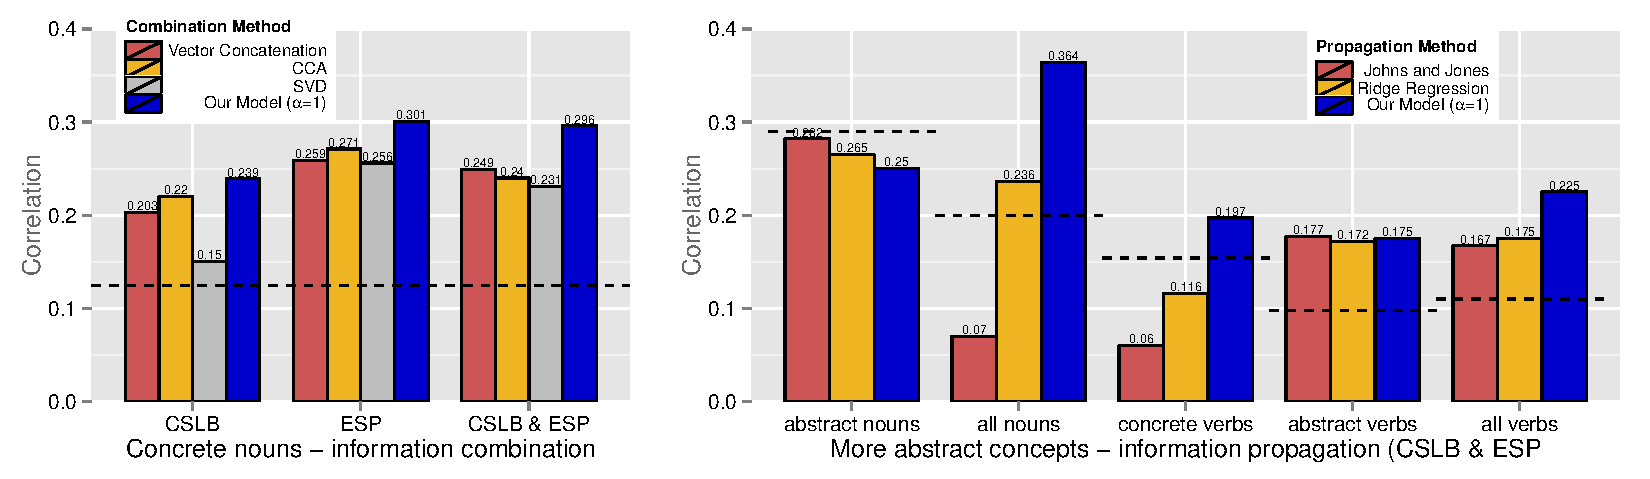
\includegraphics[width = \textwidth]{Graph_1}  \caption{The proposed approach compared with other methods of information combination (left) and propagation. Dashed lines indicate language-only model baseline.}\end{figure*}

Figure 3 (right side) illustrates the propagation performance of the three models. While the correlations overall may seem somewhat low, this is a consequence of the difficulty of modeling the USF data. In fact, the performance of both the language-only model and our multi-modal extension across the concept types, ranging from .18--.36, is equal to or higher than equivalent models evaluated on the same data previously \cite{feng2010visual,silberer2012grounded,silberer2013models}. 

For learning representations of concrete verbs, our approach achieves a 69\% increase in performance over the next best alternative. The performance of the model on abstract verbs is marginally inferior to Johns and Jones' method. Nevertheless, the clear advantage for concrete verbs makes our model the best choice for learning representations of verbs in general, as shown by performance on the set \emph{all verbs}, which also includes mixed abstract-concrete pairs. 

Our model is also marginally inferior to alternative approaches in learning representations of abstract nouns. However, in this case, no method improves on the linguistic-only baseline. It is possible that perceptual information is simply so removed from the core semantics of these concepts that they are best acquired via the linguistic medium alone, regardless of learning mechanism. The moderately inferior performance of our method in such cases is likely caused by its greater inherent inter-modal dependence compared with methods that simply concatenate uni-modal representations. When the perceptual signal is of low quality, this greater inter-modal dependence allows the linguistic signal to be obscured. The trade-off, however, is the higher quality joint representations when the perceptual signal is of higher-quality, exemplified by the fact that our proposed approach outperforms alternatives on the set \emph{all nouns}, which includes the more concrete nouns. 

\subsection{Direct representation vs. propagation}

 \begin{figure*}[t] 

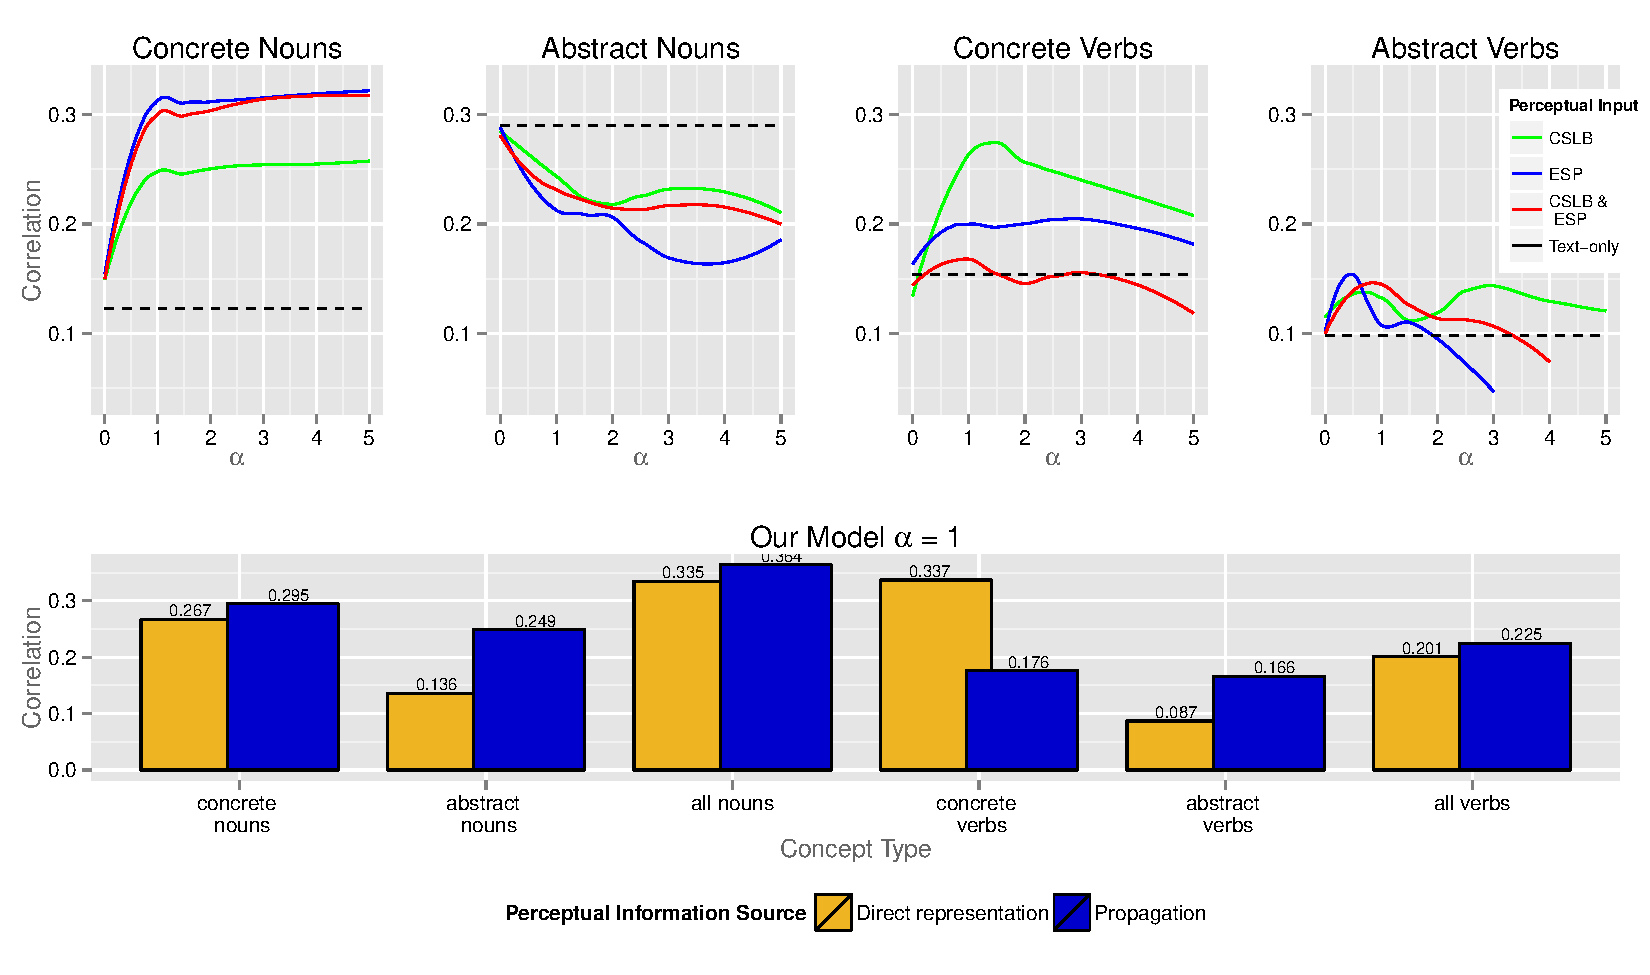
\includegraphics[width = \textwidth]{Graph_2}  

\caption{Top: Comparing the strategy of directly representing abstract concepts from perceptual information where available (yellow bars) vs. propagating via concrete concepts. Bottom: The effect of increasing \(\alpha\) on correlation with USF pairs (Spearman \(\rho\)) for each concept type. Horizontal dashed lines indicate language-only model baseline.}

\end{figure*}

Although property norm datasets such as the CSLB data typically consist of perceptual feature information for concrete nouns only, image-based datasets such as ESP do contain information on more abstract concepts, which was omitted from the previous experiments. Indeed, image banks such as Google Images contain millions of photographs portraying quite abstract concepts, such as \emph{love} or \emph{war}. On the other hand, encodings or descriptions of abstract concepts are generally more subjective and less reliable than those of concrete concepts \cite{katja2005content}. We therefore investigated whether or not it is preferable to include this additional information as model input or to restrict perceptual input to concrete nouns as previously.    

Of our evaluation sets, it was possible to construct from ESP (and add to \(\mathbf{P_{ESP}}\)) representations for all of the concrete verbs, and for approximately half of the abstract verbs and abstract nouns. Figure 4 (top), shows the performance of a our model trained on all available perceptual input versus the model in which the perceptual input was restricted to concrete nouns. 

The results reflect a clear manifestation of the abstract/concrete distinction. Concrete verbs behave similarly to concrete nouns, in that they can be effectively represented directly from perceptual information sources. The information encoded in these representations is beneficial to the model and increases performance. In contrast, constructing `perceptual' representations of abstract verbs and abstract nouns directly from perceptual information sources is clearly counter-productive (to the extent that performance also degrades on the combined sets \emph{all nouns} and \emph{all verbs}). It appears in these cases that the perceptual input acts to obscure or contradict the otherwise useful signal inferred from the corpus.

As shown in the previous section, the inclusion of any form of perceptual input inhibits the learning of abstract nouns. However, this is not the case for abstract verbs. Our model learns higher quality representations of abstract verbs when perceptual input is restricted to concrete nouns than when no perceptual input is included whatsoever \emph{and} when perceptual input is included for both concrete nouns and abstract verbs. This supports the idea of a gradual scale of concreteness: the most concrete concepts can be effectively represented directly in the perceptual modality; somewhat more abstract concepts cannot be represented directly in the perceptual modality, but have representations that are improved by propagating perceptual input from concrete concepts via language; and the most abstract concepts are best acquired via language alone.   

\subsection{Source and quantity of perceptual input} For different concept types, we tested the effect of varying the proportion of perceptual to linguistic input (the parameter \(\alpha\)). Perceptual input was restricted to concrete nouns as in Sections 3.1-3.2. 

As shown in Figure 4, performance on concrete nouns improves (albeit to a decreasing degree) as \( \alpha \) increases. When learning concrete noun representations, linguistic input is apparently redundant if perceptual input is of sufficient quality and quantity. For the other concept types, in each case there is an optimal value for \( \alpha \) in the range .5--2, above which perceptual input obscures the linguistic signal and performance degrades. The proximity of these optima to 1 suggests that  for optimal learning, when a concrete concept is experienced approximately equal weight should be given to available perceptual and linguistic information. 

\section{Conclusions}

Motivated by the notable prevalence of abstract concepts in everyday language, and their likely importance to flexible, general-purpose representation learning, we have investigated how abstract and concrete representations can be acquired by multi-modal models. In doing so, we presented a simple and easy-to-implement architecture for acquiring semantic representations of both types of concept from linguistic and perceptual input. 

While neuro-probabilistic models have been applied to the problem of multi-modal representation learning previously \cite{srivastava2012multimodal,wu2013online} our model and experiments develop this work in several important ways. First, we address the problem of learning abstract concepts. By isolating concepts of different concreteness and part-of-speech in our evaluation sets, and separating the processes of information combination and propagation, we demonstrate that the multi-modal approach is indeed effective for some, but perhaps not all, abstract concepts. In addition, our model introduces a clear parallel with human language learning. Perceptual input is introduced precisely when concrete concepts are `experienced' by the model in the corpus text, much like a language learner experiencing concrete entities via sensory perception.  

Taken together, our findings indicate the utility of distinguishing three concept types when learning representations in the multi-modal setting. 

\paragraph{Type I}Concepts that can be effectively represented directly in the perceptual modality. For such concepts, generally concrete nouns or concrete verbs, our proposed approach provides a simple means of combining perceptual and linguistic input. The resulting multi-modal representations are of higher quality than those learned via other approaches, resulting in a performance improvement of over 10\% in modelling free association.

\paragraph{Type II}Concepts, including abstract verbs, that cannot be effectively represented directly in the perceptual modality, but whose representations can be improved by joint learning from linguistic input and perceptual information about related concepts. Our model can effectively propagate perceptual input (exploiting the relations inferred from the linguistic input) from Type I concepts to enhance the representations of Type II concepts above the language-only baseline. Because of the frequency of abstract concepts, such propagation extends the benefit of the multi-modal approach to a far wider range of language than models based solely in the concrete domain. 

\paragraph{Type III}Concepts, such as abstract nouns, which are more effectively learned via language-only models than multi-modal models. Neither the model we introduce here nor other proposed propagation methods achieve an improvement in representation quality for these concepts over the language-only baseline. Of course, it is an empirical question whether a multi-modal approach could ever enhance the representation learning of these concepts, one with potential implications for cognitive theories of grounding (a topic of much debate in psychology \cite{grafton2009embodied,barsalou2010grounded}). 

Additionally, we investigated the optimum type and quantity of perceptual input for learning concepts of different types. We showed that too much perceptual input can result in degraded representations. For concepts of type I and II, the optimal quantity resulted from setting \(\alpha = 1\); i.e. whenever a concrete concept was encountered, the model learned from an equal number of language-based and perception-based examples. While we make no formal claims here, such observations may ultimately provide insight into human language learning and semantic memory. 

In future we will address the question of whether Type III concepts can ever be enhanced via multi-modal learning, and investigate multi-modal models that optimally learn concepts of each type. This may involve filtering the perceptual input stream for concepts according to concreteness, and possibly more elaborate model architectures that facilitate distinct representational frameworks for abstract and concrete concepts.

 




% include your own bib file like this:

\bibliographystyle{acl2014}

\bibliography{EMNLP2014}







\end{document}

